
\chapter[Sóng điện từ và truyền sóng điện từ]{Sóng điện từ và truyền sóng điện từ}
\section{Lý thuyết}
\subsection{Định nghĩa}
Sóng điện từ là điện từ trường lan truyền trong không gian.
\subsection {Đặc điểm}
\begin{itemize}
	\item Sóng điện từ là sóng ngang, lan truyền được trong chân không và trong các môi trường vật chất.
	\item Tốc độ truyền sóng điện từ phụ thuộc vào môi trường truyền sóng; trong chân không, không khí là $c=3\cdot 10^8\ \text{m/s}$, trong các môi trường khác, tốc độ nhỏ hơn.
	\item Vectơ cường độ điện trường $\vec{E}$ và vectơ cảm ứng từ $\vec {B}$ luôn luôn vuông góc với nhau và vuông góc với phương truyền sóng. Ba vectơ $\vec{E}, \vec{B}$ và $\vec{v}$ tại mọi điểm tạo với nhau thành một tam diện thuận.
	\begin{center}
		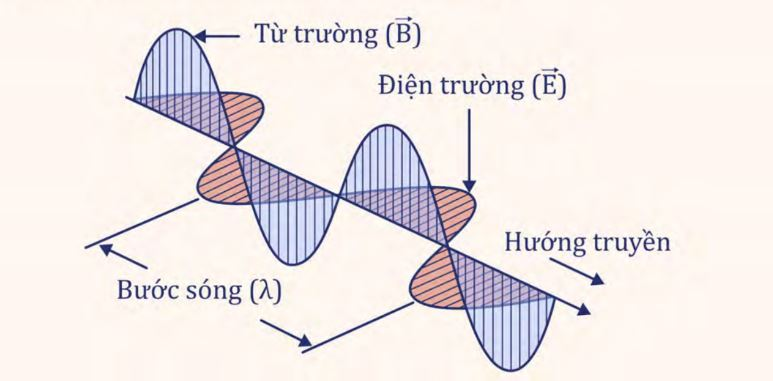
\includegraphics[scale=0.7]{../figs/4-3-1.JPG}
	\end{center}
	\item Dao động của điện trường và của từ trường tại một điểm luôn luôn cùng pha với nhau.
	\item Sóng điện từ tuân theo định luật truyền thẳng, phản xạ, khúc xạ như ánh sáng.
	\item Sóng điện từ mang năng lượng.
	\subsection {Bảng sóng vô tuyến và ứng dụng}
	\begin{tabular}{|m{2cm}|m{2.5cm}|m{13em}|m{8em}|}
		\hline
		\thead{Loại sóng} & \thead{Bước sóng}  & \thead{Đặc điểm}  & \thead{Ứng dụng}  \\
		\hline
		\nfhead{Sóng dài}	& \nfhead{$\geq 1000\ \text{m}$} & Có năng lượng thấp.\newline Bị các vật trên mặt đất hấp thụ mạnh nhưng nước lại hấp thụ ít. & Dùng trong thông tin liên lạc dưới nước. \\
		\hline
		Sóng trung	&$100-1000\ \text{m}$  & Ban ngày bị tầng điện li hấp thụ mạnh nên không truyền đi xa được. \newline Ban đêm bị tầng điện li phản xạ nên truyền đi xa được.  & Dùng trong thông tin liên lạc vào ban đêm. \\
		\hline
		Sóng ngắn	& \nfhead{$10-100\ \text{m}$}  & Có năng lượng lớn. \newline Bị phản xạ nhiều lần giữa tầng điện li và mặt đất.  & Dùng trong thông tin liên lạc trên mặt đất.  \\
		\hline
		\nfhead{Sóng cực ngắn}	&\nfhead{$1-10\ \text{m}$}  &Có năng lượng rất lớn. Không bị tầng điện li hấp thụ hay phản xạ.\newline Xuyên qua tầng điện li vào vũ trụ.  & Dùng trong thông tin vũ trụ. \\
		\hline
	\end{tabular}
\end{itemize}
\section{Bài tập tự luyện}
\begin{enumerate}[label=\bfseries Câu \arabic*:]
	\item \mkstar{1} [9] %Cau 1
	\cauhoi
	{Đặc điểm không phải đặc điểm chung của sóng cơ và sóng điện từ là
		\begin{mcq} (2)
			\item là sóng ngang.
			\item truyền được trong chân không.
			\item bị nhiễu xạ khi gặp vật cản.
			\item mang năng lượng
		\end{mcq}
	}
	
	\loigiai
	{		\textbf{Đáp án: B.}
		
		Sóng cơ không truyền được trong chân không.
		
	}
	
	%=======================	
	\item \mkstar{1} [3] %Cau 11
	\cauhoi
	{Trong sóng điện từ, điện trường và từ trường tại một điểm luôn dao động
		\begin{mcq}(2)
			\item lệch pha nhau $\dfrac{\pi}{4}$.
			\item cùng pha nhau.
			\item lệch pha nhau $\dfrac{\pi}{2}$.
			\item ngược pha nhau.
		\end{mcq}
	}
	
	\loigiai
	{		\textbf{Đáp án: B.}
		
		Trong sóng điện từ, điện trường và từ trường tại một điểm luôn dao động cùng pha nhau.
		
	}
	
	%=======================	
	\item \mkstar{1} [7] %Cau 3
	\cauhoi
	{Sóng điện từ
		\begin{mcq}(1)
			\item có điện trường và từ trường tại một điểm dao động cùng phương. 
			\item là sóng dọc hoặc sóng ngang tùy vào môi trường truyền sóng.
			\item không truyền được trong chân không.
			\item là điện từ trường lan truyền trong không gian theo thời gian.
		\end{mcq}
	}
	
	\loigiai
	{		\textbf{Đáp án: D.}
		
		Sóng điện từ là điện từ trường lan truyền trong không gian theo thời gian.
		
	}
	
	%=======================	
	\item \mkstar{1} [7] %Cau 4
	\cauhoi
	{Một sóng điện từ có tần số $\SI{100}{MHz}$ truyền với tốc độ $\xsi{3\cdot 10^{8}}{m/s}$ có bước sóng là
		\begin{mcq}(4)
			\item $\SI{0,3}{m}$ 
			\item $\SI{3}{m}$. 
			\item $\SI{30}{m}$. 
			\item $\SI{300}{m}$. 
		\end{mcq}
	}
	
	\loigiai
	{		\textbf{Đáp án: B.}
		
		Bước sóng của sóng điện từ cho bởi:
		$$
		\lambda = \dfrac{v}{f} = \dfrac{3.10^{8}}{100.10^{6}} = \SI{3}{m}.
		$$
	}
	
	%=======================	
	\item \mkstar{1} [12] %Cau 5
	\cauhoi
	{Sóng điện từ là 
		\begin{mcq}(1)
			\item điện từ trường lan truyền trong không gian.         
			\item sóng cơ và truyền được trong chất lỏng.
			\item sóng dọc và truyền được trong chân không.  
			\item sóng ngang và không thể truyền trong chân không.
		\end{mcq}
	}
	
	\loigiai
	{		\textbf{Đáp án: A.}
		
		Sóng điện từ là điện từ trường lan truyền trong không gian.   
	}
	
	%=======================
	\item \mkstar{1} [10] %Cau 6
	\cauhoi
	{Sóng điện từ
		\begin{mcq}(1)
			\item là sóng dọc hoặc sóng ngang.
			\item là điện từ trường lan truyền trong không gian.
			\item có thành phần điện trường và thành phần từ trường tại một điểm dao động cùng phương.
			\item không truyền được trong chân không.
		\end{mcq}
	}
	
	\loigiai
	{		\textbf{Đáp án: B.}
		
		Sóng điện từ à điện từ trường lan truyền trong không gian.
		
	}
	
	%=======================
	\item \mkstar{1} [4] %Cau 7
	\cauhoi
	{Khi nói về sóng điện từ, phát biểu nào sau đây là sai?
		\begin{mcq}(1)
			\item Sóng điện từ mang năng lượng. 
			\item Sóng điện từ tuân theo các quy luật giao thoa, nhiễu xạ. 
			\item Sóng điện từ là sóng ngang. 
			\item Sóng điện từ không truyền được trong chân không.
		\end{mcq}
	}
	
	\loigiai
	{		\textbf{Đáp án: D.}
		
		Sóng điện từ truyền được trong chân không.
		
	}
	
	%=======================		
	\item \mkstar{1} [7] % Cau 8
	\cauhoi
	{Đối với sự lan truyền sóng điện từ thì
		\begin{mcq}(1)
			\item vectơ cường độ điện trường cùng phương với phương truyền sóng còn vectơ cảm ứng từ vuông góc với vectơ cường độ điện trường.
			\item vectơ cảm ứng từ cùng phương với phương truyền sóng còn vectơ cường độ điện trường vuông góc với vectơ cảm ứng từ. 
			\item vectơ cường độ điện trường và vectơ cảm ứng từ luôn vuông góc với phương truyền sóng.
			\item vectơ cường độ điện trường và vectơ cảm ứng từ luôn cùng phương với phương truyền sóng.
		\end{mcq}
	}
	
	\loigiai
	{		\textbf{Đáp án: C.}
		
		Đối với sự lan truyền sóng điện từ thì vectơ cường độ điện trường và vectơ cảm ứng từ luôn vuông góc với phương truyền sóng.
		
	}
	
	%=======================
	\item \mkstar{1} [2] %Cau 9
	\cauhoi
	{Sóng điện từ được dùng trong lò vi ba (vi sóng) để hâm nóng, nấu chín thức ăn là
		\begin{mcq}(4)
			\item tia tử ngoại. 
			\item sóng cực ngắn. 
			\item tia hồng ngoại. 
			\item sóng ngắn. 
		\end{mcq}
	}
	
	\loigiai
	{		\textbf{Đáp án: B.}
		
		Sóng điện từ được dùng trong lò vi ba (vi sóng) để hâm nóng, nấu chín thức ăn là sóng cực ngắn.
		
	}
	
	%=======================
	\item \mkstar{1} [3] %Cau 10
	\cauhoi
	{Trong chân không, các bức xạ được sắp xếp theo tần số tăng dần là
		\begin{mcq}(1)
			\item Tia hồng ngoại, ánh sáng tím, tia tử ngoại, tia Rơn-ghen.
			\item Ánh sáng tím, tia hồng ngoại, tia tử ngoại, tia Rơn-ghen. 
			\item Tia Rơn-ghen, tia tử ngoại, ánh sáng tím, tia hồng ngoại. 
			\item Tia hồng ngoại, ánh sáng tím, tia Rơn-ghen, tia tử ngoại.
		\end{mcq}
	}
	
	\loigiai
	{		\textbf{Đáp án: A.}
		
		Trong chân không, các bức xạ được sắp xếp theo tần số tăng dần là tia hồng ngoại, ánh sáng tím, tia tử ngoại, tia Rơn-ghen.
		
	}
	
	%=======================	
	\item \mkstar{2} [7] %Cau 2
	\cauhoi
	{Một sóng điện từ truyền qua điểm M trong không gian. Cường độ điện trường và cảm ứng từ tại M biến thiên điều hòa với giá trị cực đại lần lượt là $E_0$ và $B_0$. Khi cảm ứng từ tại M bằng $ 0,5B_0$ thì cường độ điện trường tại đó có độ lớn là
		\begin{mcq}(4)
			\item $2E_0$.
			\item $E_0$.
			\item $0,25E_0$. 
			\item $0,5E_0$. 
		\end{mcq}
	}
	
	\loigiai
	{		\textbf{Đáp án: D.}
		
		Vì điện trường và từ trường cùng pha nên khi cảm ứng từ bằng $0,5B_0$ thì cường độ cũng điện trường bằng $0,5E_0$.
		
	}
	
	
	%=======================	
	\item \mkstar{2} [3]
	\cauhoi
	{Một sóng điện từ có tần  số $\xsi{15\cdot 10^{6}}{Hz}$ truyền trong môi trường với tốc độ $\xsi{2,25\cdot 10^{8}}{m/s}$. Trong môi trường đó, sóng điện từ có bước sóng là
		\begin{mcq}(4)
			\item $\SI{45}{m}$.
			\item $\SI{15}{m}$.
			\item $\SI{7,5}{m}$.
			\item $\SI{6,7}{m}$. 
		\end{mcq}
	}
	
	\loigiai
	{		\textbf{Đáp án: B.}
		
		Bước sóng của sóng điện từ cho bởi
		$$
		\lambda=\dfrac{v}{f}= \SI{15}{m}.
		$$
		
	}
	
	%=======================	
	\item \mkstar{3} [3]
	
	\cauhoi
	{Tại một điểm có sóng điện từ truyền qua, cường độ điện tường biến thiên theo phương trình $E=E_{0} \cos \left(2 \pi \cdot 10^{8} t-\dfrac{2 \pi}{3}\right)$ $(E_{0}>0, t$ tính bằng $s$). Kể từ lúc $t=0$, thời điểm đầu tiên để cảm ứng từ tại điểm đó bằng không là
		\begin{mcq}(4)
			\item $\xsi{\dfrac{10^{-8}}{9}}{s}$.
			\item $\xsi{\dfrac{10^{-8}}{12}}{s}$.
			\item $\xsi{\dfrac{10^{-8}}{8}}{s}$.
			\item $\xsi{\dfrac{10^{-8}}{6}}{s}$.
		\end{mcq}
	}
	
	\loigiai
	{		\textbf{Đáp án: B.}
		
		Chu kì của sóng điện từ cho bởi
		$$
		T=\dfrac{2 \pi}{\omega}=\dfrac{2 \pi}{2 \pi \cdot 10^{8}}= \xsi{10^{-8}}{s}.
		$$
		Vì cảm ứng từ và cường độ điện trường luôn cùng pha nhau, nên thời điểm đầu tiên cảm ứng từ bằng không cũng chính là thời điểm đầu tiên cường độ điện trường bằng không.
		
		Từ đường tròn pha, ta xác định được thời điểm đầu tiên cường độ điện trường bằng không cho bởi:
		$$
		t=\dfrac{T}{12}= \xsi{\dfrac{10^{-8}}{12}}{s}.
		$$
	}
		\item \mkstar{1} 
	\cauhoi
	{Mạch chọn sóng của máy thu vô tuyến điện gồm tụ điện $C = \SI{880}{pF}$ và cuộn cảm $L = \SI{20}{\mu H}$. Bước sóng điện từ mà mạch thu được là
		
		\begin{mcq}(2)
			\item $\lambda = \SI{100}{m}.$
			\item $\lambda = \SI{150}{m}.$
			\item $\lambda = \SI{250}{m}.$ 
			\item $\lambda = \SI{500}{m}.$
		\end{mcq}
	}
	
	\loigiai
	{		\textbf{Đáp án: C.}
		
	
	}
		\item \mkstar{2} 
	\cauhoi
	{Một máy thu thanh đang thu sóng ngắn. Để chuyển sang thu sóng trung, có thể thực hiện giải pháp nào sau đây trong mạch dao động anten?
		\begin{mcq}
			\item Giảm $C$ và giảm $L$.
			\item Giữ nguyên $C$ và giảm $L$.
			\item Tăng $L$ và tăng $C$. 
			\item Giữ nguyên $L$ và giảm $C$.
			
		\end{mcq}
	}
	
	\loigiai
	{		\textbf{Đáp án: C.}
		
		Để thu được sóng trung thì phải tăng bước sóng. Cần tăng $L$ giữ nguyên $C$ hoặc tăng $C$ giữ nguyên $L$ hoặc tăng cả hai.
	}
		\item \mkstar{2} 
	\cauhoi
	{Mạch chọn sóng của một máy thu thanh gồm một cuộn dây thuần cảm và một tụ điện có điện dung biến đổi được. Khi đặt điện dung của tụ điện có giá trị $\SI{20}{F}$ thì bắt được sóng có bước sóng $\SI{30}{m}$. Khi điện dung của tụ điện giá trị $\SI{180}{F}$ thì sẽ bắt được sóng có bước sóng là
		
		\begin{mcq}(4)
			\item $\lambda = \SI{150}{m}.$
			\item $\lambda = \SI{270}{m}.$
			\item $\lambda = \SI{90}{m}.$
			\item $\lambda = \SI{10}{m}.$
		\end{mcq}
	}
	
	\loigiai
	{		\textbf{Đáp án: C.}
		
		
	}
		\item \mkstar{2} 
	\cauhoi
	{Mạch chọn sóng của một máy thu vô tuyến điện gồm một tụ điện có điện dung $C = \SI{0,1}{nF}$ và cuộn cảm có độ tự cảm $L = \SI{30}{\mu H}$.  Mạch dao động trên có thể bắt được sóng vô tuyến thuộc dải
		\begin{mcq}(4)
			\item sóng trung. 
			\item sóng dài. 
			\item sóng ngắn. 
			\item sóng cực ngắn.
		\end{mcq}
	}
	
	\loigiai
	{		\textbf{Đáp án: A.}
		
		
	}
		\item \mkstar{1} 
	\cauhoi
	{Mạch chọn sóng của một máy thu gồm một tụ điện có điện dung $C= \dfrac{4}{9\pi^2}\ \text{pF}$ và cuộn cảm có độ tụ cảm biến thiên. Để có thể bắt được sóng điện từ có bước sóng $\lambda = \SI{100}{m}$ thì độ tự cảm cuộn dây bằng bao nhiêu?
		
		\begin{mcq}(4)
			\item $L = \SI{0,0645}{H}.$
			\item $L = \SI{0,0625}{H}.$
			\item $L = \SI{0,0615}{H}.$
			\item $L = \SI{0,0635}{H}.$
		\end{mcq}
	}
	
	\loigiai
	{		\textbf{Đáp án: B.}
		
		
	}
\end{enumerate}

